% !TeX spellcheck = en_US
\subsection{Method of development}
% 3 pages
We like the SCRUM development method, but have decided only to do some of the SCRUM activities. \textit{Why?}

A SCRUM activity we have chosen to exclude among others is the Daily SCRUM meeting.
At the Daily SCRUM meeting the development team and the SCRUM-master is updated with progress and set-backs.
We are a small group of only 5 people, however, and we do not have people to fill out all roles used in proper SCRUM, such as product owner and stake holders - we are only able to represent the development team.
As development will be done with the group assembled, we see no need for spending 15 minutes every meeting updating each other, as we already do this ad hoc when we are working.
The API we have defined and the SCRUM backlog should be enough to make the progress visible to all team members.

\begin{figure}[H]
  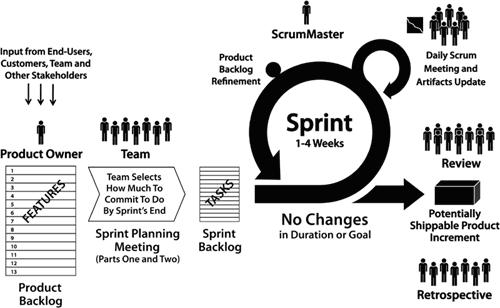
\includegraphics[width=\textwidth]{illustrations/scrum.jpg}
  \caption{SCRUM illustrated}
  \label{scrum_picture}
\end{figure}

As just mentioned, we have decided to use a backlog, which is another SCRUM artifact.
The backlog is a prioritized list of items, where each item describes a program feature, often called a `story', possibly with sub-tasks that needs to be completed. Traditionally the product owner defines the order of the items, putting the features he wants implemented first at the top of the list \cite[p. 12]{scrum-org-guide}.
We have chosen to use a backlog as it ensures that the most vital functionality is implemented over less important, nice-to-have features. We will also benefit from producing the backlog itself, as we will be forced into enumerating all features to implement, giving us an overview of the work and ensuring that no big task suddenly pops up later.
Our complete backlog can be viewed in \atref{backlog}.

We have chosen not to divide our project into sprints, even though they are a core foundation of SCRUM.
Sprints are great for projects with a longer time spans than ours, as it divides the project into smaller iterations, each producing valuable functionality able to function on its own, making it easier to keep focus.
After every sprint, the SCRUM team do a review, a retrospective, and plan which backlog items to implement during for the next sprint \cite[p. 8]{scrum-org-guide}.
Were we to divide our project into sprints, it would be very short ones, and it would not be worth the overhead from managing sprint backlogs and during reviews and retrospectives.

The SCRUM Task Board is used to overview the progress of a sprint. The board is divided into three parts; `not started',`in progress', and `complete', with the tasks of the sprint listed under the appropriate section. Often a physical board is used, with post-its representing tasks, the reason for it to be a physical board is that everybody should be able to see it all the time. This is not possible if not all are at the same location and it can be difficult if you do not have a specific location available for the duration of a sprint, which is why some choose to use a software version of the tool as we have. When a task is started it is moved from `not started' to `in progress', when a task is finished and passed its tests it is moved to `complete'. Since we in our project only have one sprint it gives an overview of the progress of the whole project and of the individual tasks.
Our task board can be viewed in \acref{taskboard}.

The burndown chart in SCRUM (as well as in other measurable environments) is used to monitor the progress of remaining task - in SCRUM this is the sprint backlog.
The burndown chart is a basic diagram where the Y-axis symbolizes the remaining work and the X-axis symbolizes the remaining time to complete the work.
At the start a line is drawn from (0,Y) to (X,0), where Y is the amount of work and X is the amount of time.
Each day the progress is plotted in with a line. This line shows the current status - and thereby maybe even the effectiveness of the team.
Since our project is a "one sprint"-project we are convinced that we can use the burndown chart to see if we are still on track. This is due to the fact that we have estimated each task, and thereby have a quite good idea of much work there is to be done and know when to be finished. When using the burndown chart we can constantly check up on our current progress and see if we are falling behind schedule.\\
Our burndown chart can be viewed in \acref{burndown}.

We will use scrumwise.com as our SCRUM tool to reduce the overhead from the above methods we have chosen to use. The overhead will be reduced, since artifacts, such as the burndown chart and the task board, automatically will be updated.
Because the various artifacts automatically are updated, we will easily be able to monitor our progress and maintain our overview. Should our work not progress as estimated and planned, we will be able to spot it immediately, and may then pause our work to reevaluate our plans, possible doing re-estimation of some or all of the tasks.